% Created by tikzDevice version 0.7.0 on 2014-06-22 22:26:53
% !TEX encoding = UTF-8 Unicode
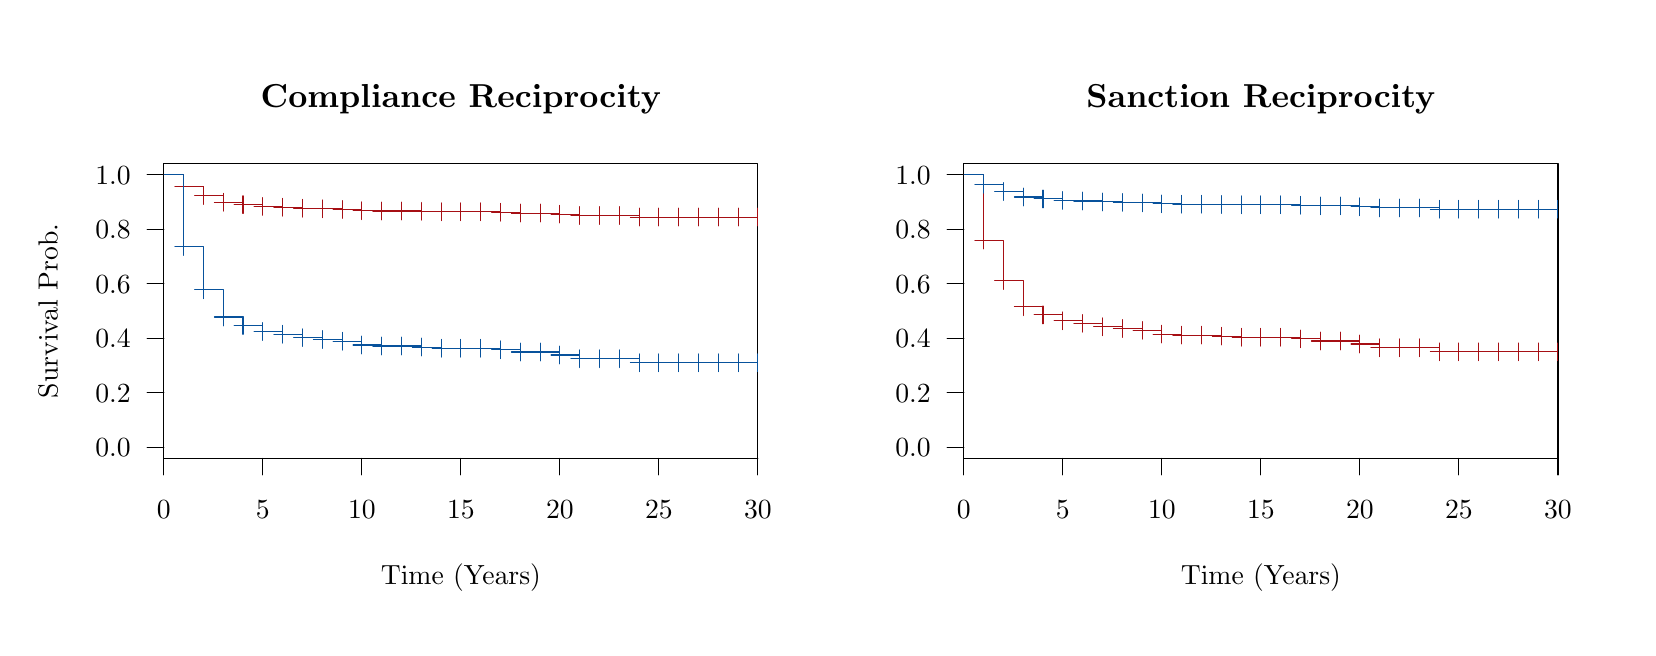
\begin{tikzpicture}[x=1pt,y=1pt]
\definecolor[named]{fillColor}{rgb}{1.00,1.00,1.00}
\path[use as bounding box,fill=fillColor,fill opacity=0.00] (0,0) rectangle (578.16,216.81);
\begin{scope}
\path[clip] (  0.00,  0.00) rectangle (578.16,216.81);
\definecolor[named]{drawColor}{rgb}{0.00,0.00,0.00}

\path[draw=drawColor,line width= 0.4pt,line join=round,line cap=round] ( 49.20, 61.20) -- (263.88, 61.20);

\path[draw=drawColor,line width= 0.4pt,line join=round,line cap=round] ( 49.20, 61.20) -- ( 49.20, 55.20);

\path[draw=drawColor,line width= 0.4pt,line join=round,line cap=round] ( 84.98, 61.20) -- ( 84.98, 55.20);

\path[draw=drawColor,line width= 0.4pt,line join=round,line cap=round] (120.76, 61.20) -- (120.76, 55.20);

\path[draw=drawColor,line width= 0.4pt,line join=round,line cap=round] (156.54, 61.20) -- (156.54, 55.20);

\path[draw=drawColor,line width= 0.4pt,line join=round,line cap=round] (192.32, 61.20) -- (192.32, 55.20);

\path[draw=drawColor,line width= 0.4pt,line join=round,line cap=round] (228.10, 61.20) -- (228.10, 55.20);

\path[draw=drawColor,line width= 0.4pt,line join=round,line cap=round] (263.88, 61.20) -- (263.88, 55.20);

\node[text=drawColor,anchor=base,inner sep=0pt, outer sep=0pt, scale=  1.00] at ( 49.20, 39.60) {0};

\node[text=drawColor,anchor=base,inner sep=0pt, outer sep=0pt, scale=  1.00] at ( 84.98, 39.60) {5};

\node[text=drawColor,anchor=base,inner sep=0pt, outer sep=0pt, scale=  1.00] at (120.76, 39.60) {10};

\node[text=drawColor,anchor=base,inner sep=0pt, outer sep=0pt, scale=  1.00] at (156.54, 39.60) {15};

\node[text=drawColor,anchor=base,inner sep=0pt, outer sep=0pt, scale=  1.00] at (192.32, 39.60) {20};

\node[text=drawColor,anchor=base,inner sep=0pt, outer sep=0pt, scale=  1.00] at (228.10, 39.60) {25};

\node[text=drawColor,anchor=base,inner sep=0pt, outer sep=0pt, scale=  1.00] at (263.88, 39.60) {30};

\path[draw=drawColor,line width= 0.4pt,line join=round,line cap=round] ( 49.20, 65.14) -- ( 49.20,163.67);

\path[draw=drawColor,line width= 0.4pt,line join=round,line cap=round] ( 49.20, 65.14) -- ( 43.20, 65.14);

\path[draw=drawColor,line width= 0.4pt,line join=round,line cap=round] ( 49.20, 84.85) -- ( 43.20, 84.85);

\path[draw=drawColor,line width= 0.4pt,line join=round,line cap=round] ( 49.20,104.55) -- ( 43.20,104.55);

\path[draw=drawColor,line width= 0.4pt,line join=round,line cap=round] ( 49.20,124.26) -- ( 43.20,124.26);

\path[draw=drawColor,line width= 0.4pt,line join=round,line cap=round] ( 49.20,143.96) -- ( 43.20,143.96);

\path[draw=drawColor,line width= 0.4pt,line join=round,line cap=round] ( 49.20,163.67) -- ( 43.20,163.67);

\node[text=drawColor,anchor=base east,inner sep=0pt, outer sep=0pt, scale=  1.00] at ( 37.20, 61.70) {0.0};

\node[text=drawColor,anchor=base east,inner sep=0pt, outer sep=0pt, scale=  1.00] at ( 37.20, 81.40) {0.2};

\node[text=drawColor,anchor=base east,inner sep=0pt, outer sep=0pt, scale=  1.00] at ( 37.20,101.11) {0.4};

\node[text=drawColor,anchor=base east,inner sep=0pt, outer sep=0pt, scale=  1.00] at ( 37.20,120.81) {0.6};

\node[text=drawColor,anchor=base east,inner sep=0pt, outer sep=0pt, scale=  1.00] at ( 37.20,140.52) {0.8};

\node[text=drawColor,anchor=base east,inner sep=0pt, outer sep=0pt, scale=  1.00] at ( 37.20,160.23) {1.0};

\path[draw=drawColor,line width= 0.4pt,line join=round,line cap=round] ( 49.20, 61.20) --
	(263.88, 61.20) --
	(263.88,167.61) --
	( 49.20,167.61) --
	( 49.20, 61.20);
\end{scope}
\begin{scope}
\path[clip] (  0.00,  0.00) rectangle (289.08,216.81);
\definecolor[named]{drawColor}{rgb}{0.00,0.00,0.00}

\node[text=drawColor,anchor=base,inner sep=0pt, outer sep=0pt, scale=  1.20] at (156.54,188.07) {\bfseries Compliance Reciprocity};
\end{scope}
\begin{scope}
\path[clip] ( 49.20, 61.20) rectangle (263.88,167.61);
\definecolor[named]{drawColor}{rgb}{0.65,0.06,0.08}

\path[draw=drawColor,line width= 0.4pt,line join=round,line cap=round] ( 49.20,163.67) --
	( 56.36,163.67) --
	( 56.36,159.42) --
	( 63.51,159.42) --
	( 63.51,156.18) --
	( 70.67,156.18) --
	( 70.67,153.72) --
	( 77.82,153.72) --
	( 77.82,152.87) --
	( 84.98,152.87) --
	( 84.98,152.22) --
	( 92.14,152.22) --
	( 92.14,151.94) --
	( 99.29,151.94) --
	( 99.29,151.55) --
	(106.45,151.55) --
	(106.45,151.35) --
	(113.60,151.35) --
	(113.60,151.13) --
	(120.76,151.13) --
	(120.76,150.68) --
	(127.92,150.68) --
	(127.92,150.56) --
	(142.23,150.56) --
	(142.23,150.44) --
	(149.38,150.44) --
	(149.38,150.30) --
	(170.85,150.30) --
	(170.85,150.10) --
	(178.01,150.10) --
	(178.01,149.82) --
	(192.32,149.82) --
	(192.32,149.43) --
	(199.48,149.43) --
	(199.48,148.94) --
	(220.94,148.94) --
	(220.94,148.37) --
	(492.87,148.37) --
	(492.87,148.37);

\path[draw=drawColor,line width= 0.4pt,line join=round,line cap=round] ( 53.17,159.42) -- ( 59.54,159.42);

\path[draw=drawColor,line width= 0.4pt,line join=round,line cap=round] ( 56.36,156.23) -- ( 56.36,162.60);

\path[draw=drawColor,line width= 0.4pt,line join=round,line cap=round] ( 60.33,156.18) -- ( 66.69,156.18);

\path[draw=drawColor,line width= 0.4pt,line join=round,line cap=round] ( 63.51,153.00) -- ( 63.51,159.36);

\path[draw=drawColor,line width= 0.4pt,line join=round,line cap=round] ( 67.49,153.72) -- ( 73.85,153.72);

\path[draw=drawColor,line width= 0.4pt,line join=round,line cap=round] ( 70.67,150.54) -- ( 70.67,156.91);

\path[draw=drawColor,line width= 0.4pt,line join=round,line cap=round] ( 74.64,152.87) -- ( 81.01,152.87);

\path[draw=drawColor,line width= 0.4pt,line join=round,line cap=round] ( 77.82,149.69) -- ( 77.82,156.05);

\path[draw=drawColor,line width= 0.4pt,line join=round,line cap=round] ( 81.80,152.22) -- ( 88.16,152.22);

\path[draw=drawColor,line width= 0.4pt,line join=round,line cap=round] ( 84.98,149.04) -- ( 84.98,155.41);

\path[draw=drawColor,line width= 0.4pt,line join=round,line cap=round] ( 88.95,151.94) -- ( 95.32,151.94);

\path[draw=drawColor,line width= 0.4pt,line join=round,line cap=round] ( 92.14,148.76) -- ( 92.14,155.12);

\path[draw=drawColor,line width= 0.4pt,line join=round,line cap=round] ( 96.11,151.55) -- (102.47,151.55);

\path[draw=drawColor,line width= 0.4pt,line join=round,line cap=round] ( 99.29,148.37) -- ( 99.29,154.73);

\path[draw=drawColor,line width= 0.4pt,line join=round,line cap=round] (103.27,151.35) -- (109.63,151.35);

\path[draw=drawColor,line width= 0.4pt,line join=round,line cap=round] (106.45,148.16) -- (106.45,154.53);

\path[draw=drawColor,line width= 0.4pt,line join=round,line cap=round] (110.42,151.13) -- (116.79,151.13);

\path[draw=drawColor,line width= 0.4pt,line join=round,line cap=round] (113.60,147.95) -- (113.60,154.31);

\path[draw=drawColor,line width= 0.4pt,line join=round,line cap=round] (117.58,150.68) -- (123.94,150.68);

\path[draw=drawColor,line width= 0.4pt,line join=round,line cap=round] (120.76,147.50) -- (120.76,153.87);

\path[draw=drawColor,line width= 0.4pt,line join=round,line cap=round] (124.73,150.56) -- (131.10,150.56);

\path[draw=drawColor,line width= 0.4pt,line join=round,line cap=round] (127.92,147.38) -- (127.92,153.75);

\path[draw=drawColor,line width= 0.4pt,line join=round,line cap=round] (131.89,150.56) -- (138.25,150.56);

\path[draw=drawColor,line width= 0.4pt,line join=round,line cap=round] (135.07,147.38) -- (135.07,153.75);

\path[draw=drawColor,line width= 0.4pt,line join=round,line cap=round] (139.05,150.44) -- (145.41,150.44);

\path[draw=drawColor,line width= 0.4pt,line join=round,line cap=round] (142.23,147.26) -- (142.23,153.62);

\path[draw=drawColor,line width= 0.4pt,line join=round,line cap=round] (146.20,150.30) -- (152.57,150.30);

\path[draw=drawColor,line width= 0.4pt,line join=round,line cap=round] (149.38,147.12) -- (149.38,153.48);

\path[draw=drawColor,line width= 0.4pt,line join=round,line cap=round] (153.36,150.30) -- (159.72,150.30);

\path[draw=drawColor,line width= 0.4pt,line join=round,line cap=round] (156.54,147.12) -- (156.54,153.48);

\path[draw=drawColor,line width= 0.4pt,line join=round,line cap=round] (160.51,150.30) -- (166.88,150.30);

\path[draw=drawColor,line width= 0.4pt,line join=round,line cap=round] (163.70,147.12) -- (163.70,153.48);

\path[draw=drawColor,line width= 0.4pt,line join=round,line cap=round] (167.67,150.10) -- (174.03,150.10);

\path[draw=drawColor,line width= 0.4pt,line join=round,line cap=round] (170.85,146.92) -- (170.85,153.28);

\path[draw=drawColor,line width= 0.4pt,line join=round,line cap=round] (174.83,149.82) -- (181.19,149.82);

\path[draw=drawColor,line width= 0.4pt,line join=round,line cap=round] (178.01,146.64) -- (178.01,153.00);

\path[draw=drawColor,line width= 0.4pt,line join=round,line cap=round] (181.98,149.82) -- (188.35,149.82);

\path[draw=drawColor,line width= 0.4pt,line join=round,line cap=round] (185.16,146.64) -- (185.16,153.00);

\path[draw=drawColor,line width= 0.4pt,line join=round,line cap=round] (189.14,149.43) -- (195.50,149.43);

\path[draw=drawColor,line width= 0.4pt,line join=round,line cap=round] (192.32,146.25) -- (192.32,152.62);

\path[draw=drawColor,line width= 0.4pt,line join=round,line cap=round] (196.29,148.94) -- (202.66,148.94);

\path[draw=drawColor,line width= 0.4pt,line join=round,line cap=round] (199.48,145.76) -- (199.48,152.12);

\path[draw=drawColor,line width= 0.4pt,line join=round,line cap=round] (203.45,148.94) -- (209.81,148.94);

\path[draw=drawColor,line width= 0.4pt,line join=round,line cap=round] (206.63,145.76) -- (206.63,152.12);

\path[draw=drawColor,line width= 0.4pt,line join=round,line cap=round] (210.61,148.94) -- (216.97,148.94);

\path[draw=drawColor,line width= 0.4pt,line join=round,line cap=round] (213.79,145.76) -- (213.79,152.12);

\path[draw=drawColor,line width= 0.4pt,line join=round,line cap=round] (217.76,148.37) -- (224.13,148.37);

\path[draw=drawColor,line width= 0.4pt,line join=round,line cap=round] (220.94,145.19) -- (220.94,151.56);

\path[draw=drawColor,line width= 0.4pt,line join=round,line cap=round] (224.92,148.37) -- (231.28,148.37);

\path[draw=drawColor,line width= 0.4pt,line join=round,line cap=round] (228.10,145.19) -- (228.10,151.56);

\path[draw=drawColor,line width= 0.4pt,line join=round,line cap=round] (232.07,148.37) -- (238.44,148.37);

\path[draw=drawColor,line width= 0.4pt,line join=round,line cap=round] (235.26,145.19) -- (235.26,151.56);

\path[draw=drawColor,line width= 0.4pt,line join=round,line cap=round] (239.23,148.37) -- (245.59,148.37);

\path[draw=drawColor,line width= 0.4pt,line join=round,line cap=round] (242.41,145.19) -- (242.41,151.56);

\path[draw=drawColor,line width= 0.4pt,line join=round,line cap=round] (246.39,148.37) -- (252.75,148.37);

\path[draw=drawColor,line width= 0.4pt,line join=round,line cap=round] (249.57,145.19) -- (249.57,151.56);

\path[draw=drawColor,line width= 0.4pt,line join=round,line cap=round] (253.54,148.37) -- (259.91,148.37);

\path[draw=drawColor,line width= 0.4pt,line join=round,line cap=round] (256.72,145.19) -- (256.72,151.56);

\path[draw=drawColor,line width= 0.4pt,line join=round,line cap=round] (260.70,148.37) -- (267.06,148.37);

\path[draw=drawColor,line width= 0.4pt,line join=round,line cap=round] (263.88,145.19) -- (263.88,151.56);

\path[draw=drawColor,line width= 0.4pt,line join=round,line cap=round] (267.85,148.37) -- (274.22,148.37);

\path[draw=drawColor,line width= 0.4pt,line join=round,line cap=round] (271.04,145.19) -- (271.04,151.56);

\path[draw=drawColor,line width= 0.4pt,line join=round,line cap=round] (275.01,148.37) -- (281.37,148.37);

\path[draw=drawColor,line width= 0.4pt,line join=round,line cap=round] (278.19,145.19) -- (278.19,151.56);

\path[draw=drawColor,line width= 0.4pt,line join=round,line cap=round] (282.17,148.37) -- (288.53,148.37);

\path[draw=drawColor,line width= 0.4pt,line join=round,line cap=round] (285.35,145.19) -- (285.35,151.56);

\path[draw=drawColor,line width= 0.4pt,line join=round,line cap=round] (289.32,148.37) -- (295.69,148.37);

\path[draw=drawColor,line width= 0.4pt,line join=round,line cap=round] (292.50,145.19) -- (292.50,151.56);

\path[draw=drawColor,line width= 0.4pt,line join=round,line cap=round] (296.48,148.37) -- (302.84,148.37);

\path[draw=drawColor,line width= 0.4pt,line join=round,line cap=round] (299.66,145.19) -- (299.66,151.56);

\path[draw=drawColor,line width= 0.4pt,line join=round,line cap=round] (303.63,148.37) -- (310.00,148.37);

\path[draw=drawColor,line width= 0.4pt,line join=round,line cap=round] (306.82,145.19) -- (306.82,151.56);

\path[draw=drawColor,line width= 0.4pt,line join=round,line cap=round] (310.79,148.37) -- (317.15,148.37);

\path[draw=drawColor,line width= 0.4pt,line join=round,line cap=round] (313.97,145.19) -- (313.97,151.56);

\path[draw=drawColor,line width= 0.4pt,line join=round,line cap=round] (317.95,148.37) -- (324.31,148.37);

\path[draw=drawColor,line width= 0.4pt,line join=round,line cap=round] (321.13,145.19) -- (321.13,151.56);

\path[draw=drawColor,line width= 0.4pt,line join=round,line cap=round] (325.10,148.37) -- (331.47,148.37);

\path[draw=drawColor,line width= 0.4pt,line join=round,line cap=round] (328.28,145.19) -- (328.28,151.56);

\path[draw=drawColor,line width= 0.4pt,line join=round,line cap=round] (332.26,148.37) -- (338.62,148.37);

\path[draw=drawColor,line width= 0.4pt,line join=round,line cap=round] (335.44,145.19) -- (335.44,151.56);

\path[draw=drawColor,line width= 0.4pt,line join=round,line cap=round] (339.41,148.37) -- (345.78,148.37);

\path[draw=drawColor,line width= 0.4pt,line join=round,line cap=round] (342.60,145.19) -- (342.60,151.56);

\path[draw=drawColor,line width= 0.4pt,line join=round,line cap=round] (346.57,148.37) -- (352.93,148.37);

\path[draw=drawColor,line width= 0.4pt,line join=round,line cap=round] (349.75,145.19) -- (349.75,151.56);

\path[draw=drawColor,line width= 0.4pt,line join=round,line cap=round] (353.73,148.37) -- (360.09,148.37);

\path[draw=drawColor,line width= 0.4pt,line join=round,line cap=round] (356.91,145.19) -- (356.91,151.56);

\path[draw=drawColor,line width= 0.4pt,line join=round,line cap=round] (360.88,148.37) -- (367.25,148.37);

\path[draw=drawColor,line width= 0.4pt,line join=round,line cap=round] (364.06,145.19) -- (364.06,151.56);

\path[draw=drawColor,line width= 0.4pt,line join=round,line cap=round] (368.04,148.37) -- (374.40,148.37);

\path[draw=drawColor,line width= 0.4pt,line join=round,line cap=round] (371.22,145.19) -- (371.22,151.56);

\path[draw=drawColor,line width= 0.4pt,line join=round,line cap=round] (375.19,148.37) -- (381.56,148.37);

\path[draw=drawColor,line width= 0.4pt,line join=round,line cap=round] (378.38,145.19) -- (378.38,151.56);

\path[draw=drawColor,line width= 0.4pt,line join=round,line cap=round] (382.35,148.37) -- (388.71,148.37);

\path[draw=drawColor,line width= 0.4pt,line join=round,line cap=round] (385.53,145.19) -- (385.53,151.56);

\path[draw=drawColor,line width= 0.4pt,line join=round,line cap=round] (389.51,148.37) -- (395.87,148.37);

\path[draw=drawColor,line width= 0.4pt,line join=round,line cap=round] (392.69,145.19) -- (392.69,151.56);

\path[draw=drawColor,line width= 0.4pt,line join=round,line cap=round] (396.66,148.37) -- (403.03,148.37);

\path[draw=drawColor,line width= 0.4pt,line join=round,line cap=round] (399.84,145.19) -- (399.84,151.56);

\path[draw=drawColor,line width= 0.4pt,line join=round,line cap=round] (403.82,148.37) -- (410.18,148.37);

\path[draw=drawColor,line width= 0.4pt,line join=round,line cap=round] (407.00,145.19) -- (407.00,151.56);

\path[draw=drawColor,line width= 0.4pt,line join=round,line cap=round] (410.97,148.37) -- (417.34,148.37);

\path[draw=drawColor,line width= 0.4pt,line join=round,line cap=round] (414.16,145.19) -- (414.16,151.56);

\path[draw=drawColor,line width= 0.4pt,line join=round,line cap=round] (418.13,148.37) -- (424.49,148.37);

\path[draw=drawColor,line width= 0.4pt,line join=round,line cap=round] (421.31,145.19) -- (421.31,151.56);

\path[draw=drawColor,line width= 0.4pt,line join=round,line cap=round] (425.29,148.37) -- (431.65,148.37);

\path[draw=drawColor,line width= 0.4pt,line join=round,line cap=round] (428.47,145.19) -- (428.47,151.56);

\path[draw=drawColor,line width= 0.4pt,line join=round,line cap=round] (432.44,148.37) -- (438.81,148.37);

\path[draw=drawColor,line width= 0.4pt,line join=round,line cap=round] (435.62,145.19) -- (435.62,151.56);

\path[draw=drawColor,line width= 0.4pt,line join=round,line cap=round] (439.60,148.37) -- (445.96,148.37);

\path[draw=drawColor,line width= 0.4pt,line join=round,line cap=round] (442.78,145.19) -- (442.78,151.56);

\path[draw=drawColor,line width= 0.4pt,line join=round,line cap=round] (446.75,148.37) -- (453.12,148.37);

\path[draw=drawColor,line width= 0.4pt,line join=round,line cap=round] (449.94,145.19) -- (449.94,151.56);

\path[draw=drawColor,line width= 0.4pt,line join=round,line cap=round] (453.91,148.37) -- (460.27,148.37);

\path[draw=drawColor,line width= 0.4pt,line join=round,line cap=round] (457.09,145.19) -- (457.09,151.56);

\path[draw=drawColor,line width= 0.4pt,line join=round,line cap=round] (461.07,148.37) -- (467.43,148.37);

\path[draw=drawColor,line width= 0.4pt,line join=round,line cap=round] (464.25,145.19) -- (464.25,151.56);

\path[draw=drawColor,line width= 0.4pt,line join=round,line cap=round] (468.22,148.37) -- (474.59,148.37);

\path[draw=drawColor,line width= 0.4pt,line join=round,line cap=round] (471.40,145.19) -- (471.40,151.56);

\path[draw=drawColor,line width= 0.4pt,line join=round,line cap=round] (475.38,148.37) -- (481.74,148.37);

\path[draw=drawColor,line width= 0.4pt,line join=round,line cap=round] (478.56,145.19) -- (478.56,151.56);

\path[draw=drawColor,line width= 0.4pt,line join=round,line cap=round] (482.53,148.37) -- (488.90,148.37);

\path[draw=drawColor,line width= 0.4pt,line join=round,line cap=round] (485.72,145.19) -- (485.72,151.56);

\path[draw=drawColor,line width= 0.4pt,line join=round,line cap=round] (489.69,148.37) -- (496.05,148.37);

\path[draw=drawColor,line width= 0.4pt,line join=round,line cap=round] (492.87,145.19) -- (492.87,151.56);
\definecolor[named]{drawColor}{rgb}{0.03,0.32,0.61}

\path[draw=drawColor,line width= 0.4pt,line join=round,line cap=round] ( 49.20,163.67) --
	( 56.36,163.67) --
	( 56.36,137.70) --
	( 63.51,137.70) --
	( 63.51,122.10) --
	( 70.67,122.10) --
	( 70.67,112.25) --
	( 77.82,112.25) --
	( 77.82,109.19) --
	( 84.98,109.19) --
	( 84.98,107.00) --
	( 92.14,107.00) --
	( 92.14,106.05) --
	( 99.29,106.05) --
	( 99.29,104.80) --
	(106.45,104.80) --
	(106.45,104.15) --
	(113.60,104.15) --
	(113.60,103.49) --
	(120.76,103.49) --
	(120.76,102.13) --
	(127.92,102.13) --
	(127.92,101.77) --
	(142.23,101.77) --
	(142.23,101.39) --
	(149.38,101.39) --
	(149.38,100.98) --
	(170.85,100.98) --
	(170.85,100.40) --
	(178.01,100.40) --
	(178.01, 99.61) --
	(192.32, 99.61) --
	(192.32, 98.54) --
	(199.48, 98.54) --
	(199.48, 97.20) --
	(220.94, 97.20) --
	(220.94, 95.73) --
	(492.87, 95.73) --
	(492.87, 95.73);

\path[draw=drawColor,line width= 0.4pt,line join=round,line cap=round] ( 53.17,137.70) -- ( 59.54,137.70);

\path[draw=drawColor,line width= 0.4pt,line join=round,line cap=round] ( 56.36,134.52) -- ( 56.36,140.89);

\path[draw=drawColor,line width= 0.4pt,line join=round,line cap=round] ( 60.33,122.10) -- ( 66.69,122.10);

\path[draw=drawColor,line width= 0.4pt,line join=round,line cap=round] ( 63.51,118.91) -- ( 63.51,125.28);

\path[draw=drawColor,line width= 0.4pt,line join=round,line cap=round] ( 67.49,112.25) -- ( 73.85,112.25);

\path[draw=drawColor,line width= 0.4pt,line join=round,line cap=round] ( 70.67,109.07) -- ( 70.67,115.44);

\path[draw=drawColor,line width= 0.4pt,line join=round,line cap=round] ( 74.64,109.19) -- ( 81.01,109.19);

\path[draw=drawColor,line width= 0.4pt,line join=round,line cap=round] ( 77.82,106.00) -- ( 77.82,112.37);

\path[draw=drawColor,line width= 0.4pt,line join=round,line cap=round] ( 81.80,107.00) -- ( 88.16,107.00);

\path[draw=drawColor,line width= 0.4pt,line join=round,line cap=round] ( 84.98,103.81) -- ( 84.98,110.18);

\path[draw=drawColor,line width= 0.4pt,line join=round,line cap=round] ( 88.95,106.05) -- ( 95.32,106.05);

\path[draw=drawColor,line width= 0.4pt,line join=round,line cap=round] ( 92.14,102.87) -- ( 92.14,109.23);

\path[draw=drawColor,line width= 0.4pt,line join=round,line cap=round] ( 96.11,104.80) -- (102.47,104.80);

\path[draw=drawColor,line width= 0.4pt,line join=round,line cap=round] ( 99.29,101.62) -- ( 99.29,107.98);

\path[draw=drawColor,line width= 0.4pt,line join=round,line cap=round] (103.27,104.15) -- (109.63,104.15);

\path[draw=drawColor,line width= 0.4pt,line join=round,line cap=round] (106.45,100.97) -- (106.45,107.34);

\path[draw=drawColor,line width= 0.4pt,line join=round,line cap=round] (110.42,103.49) -- (116.79,103.49);

\path[draw=drawColor,line width= 0.4pt,line join=round,line cap=round] (113.60,100.30) -- (113.60,106.67);

\path[draw=drawColor,line width= 0.4pt,line join=round,line cap=round] (117.58,102.13) -- (123.94,102.13);

\path[draw=drawColor,line width= 0.4pt,line join=round,line cap=round] (120.76, 98.95) -- (120.76,105.31);

\path[draw=drawColor,line width= 0.4pt,line join=round,line cap=round] (124.73,101.77) -- (131.10,101.77);

\path[draw=drawColor,line width= 0.4pt,line join=round,line cap=round] (127.92, 98.59) -- (127.92,104.95);

\path[draw=drawColor,line width= 0.4pt,line join=round,line cap=round] (131.89,101.77) -- (138.25,101.77);

\path[draw=drawColor,line width= 0.4pt,line join=round,line cap=round] (135.07, 98.59) -- (135.07,104.95);

\path[draw=drawColor,line width= 0.4pt,line join=round,line cap=round] (139.05,101.39) -- (145.41,101.39);

\path[draw=drawColor,line width= 0.4pt,line join=round,line cap=round] (142.23, 98.21) -- (142.23,104.58);

\path[draw=drawColor,line width= 0.4pt,line join=round,line cap=round] (146.20,100.98) -- (152.57,100.98);

\path[draw=drawColor,line width= 0.4pt,line join=round,line cap=round] (149.38, 97.80) -- (149.38,104.17);

\path[draw=drawColor,line width= 0.4pt,line join=round,line cap=round] (153.36,100.98) -- (159.72,100.98);

\path[draw=drawColor,line width= 0.4pt,line join=round,line cap=round] (156.54, 97.80) -- (156.54,104.17);

\path[draw=drawColor,line width= 0.4pt,line join=round,line cap=round] (160.51,100.98) -- (166.88,100.98);

\path[draw=drawColor,line width= 0.4pt,line join=round,line cap=round] (163.70, 97.80) -- (163.70,104.17);

\path[draw=drawColor,line width= 0.4pt,line join=round,line cap=round] (167.67,100.40) -- (174.03,100.40);

\path[draw=drawColor,line width= 0.4pt,line join=round,line cap=round] (170.85, 97.22) -- (170.85,103.59);

\path[draw=drawColor,line width= 0.4pt,line join=round,line cap=round] (174.83, 99.61) -- (181.19, 99.61);

\path[draw=drawColor,line width= 0.4pt,line join=round,line cap=round] (178.01, 96.43) -- (178.01,102.80);

\path[draw=drawColor,line width= 0.4pt,line join=round,line cap=round] (181.98, 99.61) -- (188.35, 99.61);

\path[draw=drawColor,line width= 0.4pt,line join=round,line cap=round] (185.16, 96.43) -- (185.16,102.80);

\path[draw=drawColor,line width= 0.4pt,line join=round,line cap=round] (189.14, 98.54) -- (195.50, 98.54);

\path[draw=drawColor,line width= 0.4pt,line join=round,line cap=round] (192.32, 95.36) -- (192.32,101.72);

\path[draw=drawColor,line width= 0.4pt,line join=round,line cap=round] (196.29, 97.20) -- (202.66, 97.20);

\path[draw=drawColor,line width= 0.4pt,line join=round,line cap=round] (199.48, 94.02) -- (199.48,100.38);

\path[draw=drawColor,line width= 0.4pt,line join=round,line cap=round] (203.45, 97.20) -- (209.81, 97.20);

\path[draw=drawColor,line width= 0.4pt,line join=round,line cap=round] (206.63, 94.02) -- (206.63,100.38);

\path[draw=drawColor,line width= 0.4pt,line join=round,line cap=round] (210.61, 97.20) -- (216.97, 97.20);

\path[draw=drawColor,line width= 0.4pt,line join=round,line cap=round] (213.79, 94.02) -- (213.79,100.38);

\path[draw=drawColor,line width= 0.4pt,line join=round,line cap=round] (217.76, 95.73) -- (224.13, 95.73);

\path[draw=drawColor,line width= 0.4pt,line join=round,line cap=round] (220.94, 92.55) -- (220.94, 98.92);

\path[draw=drawColor,line width= 0.4pt,line join=round,line cap=round] (224.92, 95.73) -- (231.28, 95.73);

\path[draw=drawColor,line width= 0.4pt,line join=round,line cap=round] (228.10, 92.55) -- (228.10, 98.92);

\path[draw=drawColor,line width= 0.4pt,line join=round,line cap=round] (232.07, 95.73) -- (238.44, 95.73);

\path[draw=drawColor,line width= 0.4pt,line join=round,line cap=round] (235.26, 92.55) -- (235.26, 98.92);

\path[draw=drawColor,line width= 0.4pt,line join=round,line cap=round] (239.23, 95.73) -- (245.59, 95.73);

\path[draw=drawColor,line width= 0.4pt,line join=round,line cap=round] (242.41, 92.55) -- (242.41, 98.92);

\path[draw=drawColor,line width= 0.4pt,line join=round,line cap=round] (246.39, 95.73) -- (252.75, 95.73);

\path[draw=drawColor,line width= 0.4pt,line join=round,line cap=round] (249.57, 92.55) -- (249.57, 98.92);

\path[draw=drawColor,line width= 0.4pt,line join=round,line cap=round] (253.54, 95.73) -- (259.91, 95.73);

\path[draw=drawColor,line width= 0.4pt,line join=round,line cap=round] (256.72, 92.55) -- (256.72, 98.92);

\path[draw=drawColor,line width= 0.4pt,line join=round,line cap=round] (260.70, 95.73) -- (267.06, 95.73);

\path[draw=drawColor,line width= 0.4pt,line join=round,line cap=round] (263.88, 92.55) -- (263.88, 98.92);

\path[draw=drawColor,line width= 0.4pt,line join=round,line cap=round] (267.85, 95.73) -- (274.22, 95.73);

\path[draw=drawColor,line width= 0.4pt,line join=round,line cap=round] (271.04, 92.55) -- (271.04, 98.92);

\path[draw=drawColor,line width= 0.4pt,line join=round,line cap=round] (275.01, 95.73) -- (281.37, 95.73);

\path[draw=drawColor,line width= 0.4pt,line join=round,line cap=round] (278.19, 92.55) -- (278.19, 98.92);

\path[draw=drawColor,line width= 0.4pt,line join=round,line cap=round] (282.17, 95.73) -- (288.53, 95.73);

\path[draw=drawColor,line width= 0.4pt,line join=round,line cap=round] (285.35, 92.55) -- (285.35, 98.92);

\path[draw=drawColor,line width= 0.4pt,line join=round,line cap=round] (289.32, 95.73) -- (295.69, 95.73);

\path[draw=drawColor,line width= 0.4pt,line join=round,line cap=round] (292.50, 92.55) -- (292.50, 98.92);

\path[draw=drawColor,line width= 0.4pt,line join=round,line cap=round] (296.48, 95.73) -- (302.84, 95.73);

\path[draw=drawColor,line width= 0.4pt,line join=round,line cap=round] (299.66, 92.55) -- (299.66, 98.92);

\path[draw=drawColor,line width= 0.4pt,line join=round,line cap=round] (303.63, 95.73) -- (310.00, 95.73);

\path[draw=drawColor,line width= 0.4pt,line join=round,line cap=round] (306.82, 92.55) -- (306.82, 98.92);

\path[draw=drawColor,line width= 0.4pt,line join=round,line cap=round] (310.79, 95.73) -- (317.15, 95.73);

\path[draw=drawColor,line width= 0.4pt,line join=round,line cap=round] (313.97, 92.55) -- (313.97, 98.92);

\path[draw=drawColor,line width= 0.4pt,line join=round,line cap=round] (317.95, 95.73) -- (324.31, 95.73);

\path[draw=drawColor,line width= 0.4pt,line join=round,line cap=round] (321.13, 92.55) -- (321.13, 98.92);

\path[draw=drawColor,line width= 0.4pt,line join=round,line cap=round] (325.10, 95.73) -- (331.47, 95.73);

\path[draw=drawColor,line width= 0.4pt,line join=round,line cap=round] (328.28, 92.55) -- (328.28, 98.92);

\path[draw=drawColor,line width= 0.4pt,line join=round,line cap=round] (332.26, 95.73) -- (338.62, 95.73);

\path[draw=drawColor,line width= 0.4pt,line join=round,line cap=round] (335.44, 92.55) -- (335.44, 98.92);

\path[draw=drawColor,line width= 0.4pt,line join=round,line cap=round] (339.41, 95.73) -- (345.78, 95.73);

\path[draw=drawColor,line width= 0.4pt,line join=round,line cap=round] (342.60, 92.55) -- (342.60, 98.92);

\path[draw=drawColor,line width= 0.4pt,line join=round,line cap=round] (346.57, 95.73) -- (352.93, 95.73);

\path[draw=drawColor,line width= 0.4pt,line join=round,line cap=round] (349.75, 92.55) -- (349.75, 98.92);

\path[draw=drawColor,line width= 0.4pt,line join=round,line cap=round] (353.73, 95.73) -- (360.09, 95.73);

\path[draw=drawColor,line width= 0.4pt,line join=round,line cap=round] (356.91, 92.55) -- (356.91, 98.92);

\path[draw=drawColor,line width= 0.4pt,line join=round,line cap=round] (360.88, 95.73) -- (367.25, 95.73);

\path[draw=drawColor,line width= 0.4pt,line join=round,line cap=round] (364.06, 92.55) -- (364.06, 98.92);

\path[draw=drawColor,line width= 0.4pt,line join=round,line cap=round] (368.04, 95.73) -- (374.40, 95.73);

\path[draw=drawColor,line width= 0.4pt,line join=round,line cap=round] (371.22, 92.55) -- (371.22, 98.92);

\path[draw=drawColor,line width= 0.4pt,line join=round,line cap=round] (375.19, 95.73) -- (381.56, 95.73);

\path[draw=drawColor,line width= 0.4pt,line join=round,line cap=round] (378.38, 92.55) -- (378.38, 98.92);

\path[draw=drawColor,line width= 0.4pt,line join=round,line cap=round] (382.35, 95.73) -- (388.71, 95.73);

\path[draw=drawColor,line width= 0.4pt,line join=round,line cap=round] (385.53, 92.55) -- (385.53, 98.92);

\path[draw=drawColor,line width= 0.4pt,line join=round,line cap=round] (389.51, 95.73) -- (395.87, 95.73);

\path[draw=drawColor,line width= 0.4pt,line join=round,line cap=round] (392.69, 92.55) -- (392.69, 98.92);

\path[draw=drawColor,line width= 0.4pt,line join=round,line cap=round] (396.66, 95.73) -- (403.03, 95.73);

\path[draw=drawColor,line width= 0.4pt,line join=round,line cap=round] (399.84, 92.55) -- (399.84, 98.92);

\path[draw=drawColor,line width= 0.4pt,line join=round,line cap=round] (403.82, 95.73) -- (410.18, 95.73);

\path[draw=drawColor,line width= 0.4pt,line join=round,line cap=round] (407.00, 92.55) -- (407.00, 98.92);

\path[draw=drawColor,line width= 0.4pt,line join=round,line cap=round] (410.97, 95.73) -- (417.34, 95.73);

\path[draw=drawColor,line width= 0.4pt,line join=round,line cap=round] (414.16, 92.55) -- (414.16, 98.92);

\path[draw=drawColor,line width= 0.4pt,line join=round,line cap=round] (418.13, 95.73) -- (424.49, 95.73);

\path[draw=drawColor,line width= 0.4pt,line join=round,line cap=round] (421.31, 92.55) -- (421.31, 98.92);

\path[draw=drawColor,line width= 0.4pt,line join=round,line cap=round] (425.29, 95.73) -- (431.65, 95.73);

\path[draw=drawColor,line width= 0.4pt,line join=round,line cap=round] (428.47, 92.55) -- (428.47, 98.92);

\path[draw=drawColor,line width= 0.4pt,line join=round,line cap=round] (432.44, 95.73) -- (438.81, 95.73);

\path[draw=drawColor,line width= 0.4pt,line join=round,line cap=round] (435.62, 92.55) -- (435.62, 98.92);

\path[draw=drawColor,line width= 0.4pt,line join=round,line cap=round] (439.60, 95.73) -- (445.96, 95.73);

\path[draw=drawColor,line width= 0.4pt,line join=round,line cap=round] (442.78, 92.55) -- (442.78, 98.92);

\path[draw=drawColor,line width= 0.4pt,line join=round,line cap=round] (446.75, 95.73) -- (453.12, 95.73);

\path[draw=drawColor,line width= 0.4pt,line join=round,line cap=round] (449.94, 92.55) -- (449.94, 98.92);

\path[draw=drawColor,line width= 0.4pt,line join=round,line cap=round] (453.91, 95.73) -- (460.27, 95.73);

\path[draw=drawColor,line width= 0.4pt,line join=round,line cap=round] (457.09, 92.55) -- (457.09, 98.92);

\path[draw=drawColor,line width= 0.4pt,line join=round,line cap=round] (461.07, 95.73) -- (467.43, 95.73);

\path[draw=drawColor,line width= 0.4pt,line join=round,line cap=round] (464.25, 92.55) -- (464.25, 98.92);

\path[draw=drawColor,line width= 0.4pt,line join=round,line cap=round] (468.22, 95.73) -- (474.59, 95.73);

\path[draw=drawColor,line width= 0.4pt,line join=round,line cap=round] (471.40, 92.55) -- (471.40, 98.92);

\path[draw=drawColor,line width= 0.4pt,line join=round,line cap=round] (475.38, 95.73) -- (481.74, 95.73);

\path[draw=drawColor,line width= 0.4pt,line join=round,line cap=round] (478.56, 92.55) -- (478.56, 98.92);

\path[draw=drawColor,line width= 0.4pt,line join=round,line cap=round] (482.53, 95.73) -- (488.90, 95.73);

\path[draw=drawColor,line width= 0.4pt,line join=round,line cap=round] (485.72, 92.55) -- (485.72, 98.92);

\path[draw=drawColor,line width= 0.4pt,line join=round,line cap=round] (489.69, 95.73) -- (496.05, 95.73);

\path[draw=drawColor,line width= 0.4pt,line join=round,line cap=round] (492.87, 92.55) -- (492.87, 98.92);
\end{scope}
\begin{scope}
\path[clip] (  0.00,  0.00) rectangle (289.08,216.81);
\definecolor[named]{drawColor}{rgb}{0.00,0.00,0.00}

\node[text=drawColor,rotate= 90.00,anchor=base,inner sep=0pt, outer sep=0pt, scale=  1.00] at ( 10.80,114.41) {Survival Prob.};

\node[text=drawColor,anchor=base,inner sep=0pt, outer sep=0pt, scale=  1.00] at (156.54, 15.60) {Time (Years)};
\end{scope}
\begin{scope}
\path[clip] (  0.00,  0.00) rectangle (578.16,216.81);
\definecolor[named]{drawColor}{rgb}{0.00,0.00,0.00}

\path[draw=drawColor,line width= 0.4pt,line join=round,line cap=round] (338.28, 61.20) -- (552.96, 61.20);

\path[draw=drawColor,line width= 0.4pt,line join=round,line cap=round] (338.28, 61.20) -- (338.28, 55.20);

\path[draw=drawColor,line width= 0.4pt,line join=round,line cap=round] (374.06, 61.20) -- (374.06, 55.20);

\path[draw=drawColor,line width= 0.4pt,line join=round,line cap=round] (409.84, 61.20) -- (409.84, 55.20);

\path[draw=drawColor,line width= 0.4pt,line join=round,line cap=round] (445.62, 61.20) -- (445.62, 55.20);

\path[draw=drawColor,line width= 0.4pt,line join=round,line cap=round] (481.40, 61.20) -- (481.40, 55.20);

\path[draw=drawColor,line width= 0.4pt,line join=round,line cap=round] (517.18, 61.20) -- (517.18, 55.20);

\path[draw=drawColor,line width= 0.4pt,line join=round,line cap=round] (552.96, 61.20) -- (552.96, 55.20);

\node[text=drawColor,anchor=base,inner sep=0pt, outer sep=0pt, scale=  1.00] at (338.28, 39.60) {0};

\node[text=drawColor,anchor=base,inner sep=0pt, outer sep=0pt, scale=  1.00] at (374.06, 39.60) {5};

\node[text=drawColor,anchor=base,inner sep=0pt, outer sep=0pt, scale=  1.00] at (409.84, 39.60) {10};

\node[text=drawColor,anchor=base,inner sep=0pt, outer sep=0pt, scale=  1.00] at (445.62, 39.60) {15};

\node[text=drawColor,anchor=base,inner sep=0pt, outer sep=0pt, scale=  1.00] at (481.40, 39.60) {20};

\node[text=drawColor,anchor=base,inner sep=0pt, outer sep=0pt, scale=  1.00] at (517.18, 39.60) {25};

\node[text=drawColor,anchor=base,inner sep=0pt, outer sep=0pt, scale=  1.00] at (552.96, 39.60) {30};

\path[draw=drawColor,line width= 0.4pt,line join=round,line cap=round] (338.28, 65.14) -- (338.28,163.67);

\path[draw=drawColor,line width= 0.4pt,line join=round,line cap=round] (338.28, 65.14) -- (332.28, 65.14);

\path[draw=drawColor,line width= 0.4pt,line join=round,line cap=round] (338.28, 84.85) -- (332.28, 84.85);

\path[draw=drawColor,line width= 0.4pt,line join=round,line cap=round] (338.28,104.55) -- (332.28,104.55);

\path[draw=drawColor,line width= 0.4pt,line join=round,line cap=round] (338.28,124.26) -- (332.28,124.26);

\path[draw=drawColor,line width= 0.4pt,line join=round,line cap=round] (338.28,143.96) -- (332.28,143.96);

\path[draw=drawColor,line width= 0.4pt,line join=round,line cap=round] (338.28,163.67) -- (332.28,163.67);

\node[text=drawColor,anchor=base east,inner sep=0pt, outer sep=0pt, scale=  1.00] at (326.28, 61.70) {0.0};

\node[text=drawColor,anchor=base east,inner sep=0pt, outer sep=0pt, scale=  1.00] at (326.28, 81.40) {0.2};

\node[text=drawColor,anchor=base east,inner sep=0pt, outer sep=0pt, scale=  1.00] at (326.28,101.11) {0.4};

\node[text=drawColor,anchor=base east,inner sep=0pt, outer sep=0pt, scale=  1.00] at (326.28,120.81) {0.6};

\node[text=drawColor,anchor=base east,inner sep=0pt, outer sep=0pt, scale=  1.00] at (326.28,140.52) {0.8};

\node[text=drawColor,anchor=base east,inner sep=0pt, outer sep=0pt, scale=  1.00] at (326.28,160.23) {1.0};

\path[draw=drawColor,line width= 0.4pt,line join=round,line cap=round] (338.28, 61.20) --
	(552.96, 61.20) --
	(552.96,167.61) --
	(338.28,167.61) --
	(338.28, 61.20);
\end{scope}
\begin{scope}
\path[clip] (289.08,  0.00) rectangle (578.16,216.81);
\definecolor[named]{drawColor}{rgb}{0.00,0.00,0.00}

\node[text=drawColor,anchor=base,inner sep=0pt, outer sep=0pt, scale=  1.20] at (445.62,188.07) {\bfseries Sanction Reciprocity};
\end{scope}
\begin{scope}
\path[clip] (338.28, 61.20) rectangle (552.96,167.61);
\definecolor[named]{drawColor}{rgb}{0.65,0.06,0.08}

\path[draw=drawColor,line width= 0.4pt,line join=round,line cap=round] (338.28,163.67) --
	(345.44,163.67) --
	(345.44,140.04) --
	(352.59,140.04) --
	(352.59,125.42) --
	(359.75,125.42) --
	(359.75,115.99) --
	(366.90,115.99) --
	(366.90,113.01) --
	(374.06,113.01) --
	(374.06,110.88) --
	(381.22,110.88) --
	(381.22,109.95) --
	(388.37,109.95) --
	(388.37,108.72) --
	(395.53,108.72) --
	(395.53,108.08) --
	(402.68,108.08) --
	(402.68,107.42) --
	(409.84,107.42) --
	(409.84,106.08) --
	(417.00,106.08) --
	(417.00,105.72) --
	(431.31,105.72) --
	(431.31,105.35) --
	(438.46,105.35) --
	(438.46,104.94) --
	(459.93,104.94) --
	(459.93,104.36) --
	(467.09,104.36) --
	(467.09,103.57) --
	(481.40,103.57) --
	(481.40,102.50) --
	(488.56,102.50) --
	(488.56,101.15) --
	(510.02,101.15) --
	(510.02, 99.67) --
	(578.16, 99.67);

\path[draw=drawColor,line width= 0.4pt,line join=round,line cap=round] (342.25,140.04) -- (348.62,140.04);

\path[draw=drawColor,line width= 0.4pt,line join=round,line cap=round] (345.44,136.86) -- (345.44,143.22);

\path[draw=drawColor,line width= 0.4pt,line join=round,line cap=round] (349.41,125.42) -- (355.77,125.42);

\path[draw=drawColor,line width= 0.4pt,line join=round,line cap=round] (352.59,122.24) -- (352.59,128.60);

\path[draw=drawColor,line width= 0.4pt,line join=round,line cap=round] (356.57,115.99) -- (362.93,115.99);

\path[draw=drawColor,line width= 0.4pt,line join=round,line cap=round] (359.75,112.81) -- (359.75,119.18);

\path[draw=drawColor,line width= 0.4pt,line join=round,line cap=round] (363.72,113.01) -- (370.09,113.01);

\path[draw=drawColor,line width= 0.4pt,line join=round,line cap=round] (366.90,109.83) -- (366.90,116.20);

\path[draw=drawColor,line width= 0.4pt,line join=round,line cap=round] (370.88,110.88) -- (377.24,110.88);

\path[draw=drawColor,line width= 0.4pt,line join=round,line cap=round] (374.06,107.69) -- (374.06,114.06);

\path[draw=drawColor,line width= 0.4pt,line join=round,line cap=round] (378.03,109.95) -- (384.40,109.95);

\path[draw=drawColor,line width= 0.4pt,line join=round,line cap=round] (381.22,106.77) -- (381.22,113.13);

\path[draw=drawColor,line width= 0.4pt,line join=round,line cap=round] (385.19,108.72) -- (391.55,108.72);

\path[draw=drawColor,line width= 0.4pt,line join=round,line cap=round] (388.37,105.54) -- (388.37,111.90);

\path[draw=drawColor,line width= 0.4pt,line join=round,line cap=round] (392.35,108.08) -- (398.71,108.08);

\path[draw=drawColor,line width= 0.4pt,line join=round,line cap=round] (395.53,104.90) -- (395.53,111.26);

\path[draw=drawColor,line width= 0.4pt,line join=round,line cap=round] (399.50,107.42) -- (405.87,107.42);

\path[draw=drawColor,line width= 0.4pt,line join=round,line cap=round] (402.68,104.24) -- (402.68,110.60);

\path[draw=drawColor,line width= 0.4pt,line join=round,line cap=round] (406.66,106.08) -- (413.02,106.08);

\path[draw=drawColor,line width= 0.4pt,line join=round,line cap=round] (409.84,102.89) -- (409.84,109.26);

\path[draw=drawColor,line width= 0.4pt,line join=round,line cap=round] (413.81,105.72) -- (420.18,105.72);

\path[draw=drawColor,line width= 0.4pt,line join=round,line cap=round] (417.00,102.54) -- (417.00,108.90);

\path[draw=drawColor,line width= 0.4pt,line join=round,line cap=round] (420.97,105.72) -- (427.33,105.72);

\path[draw=drawColor,line width= 0.4pt,line join=round,line cap=round] (424.15,102.54) -- (424.15,108.90);

\path[draw=drawColor,line width= 0.4pt,line join=round,line cap=round] (428.13,105.35) -- (434.49,105.35);

\path[draw=drawColor,line width= 0.4pt,line join=round,line cap=round] (431.31,102.17) -- (431.31,108.53);

\path[draw=drawColor,line width= 0.4pt,line join=round,line cap=round] (435.28,104.94) -- (441.65,104.94);

\path[draw=drawColor,line width= 0.4pt,line join=round,line cap=round] (438.46,101.76) -- (438.46,108.12);

\path[draw=drawColor,line width= 0.4pt,line join=round,line cap=round] (442.44,104.94) -- (448.80,104.94);

\path[draw=drawColor,line width= 0.4pt,line join=round,line cap=round] (445.62,101.76) -- (445.62,108.12);

\path[draw=drawColor,line width= 0.4pt,line join=round,line cap=round] (449.59,104.94) -- (455.96,104.94);

\path[draw=drawColor,line width= 0.4pt,line join=round,line cap=round] (452.78,101.76) -- (452.78,108.12);

\path[draw=drawColor,line width= 0.4pt,line join=round,line cap=round] (456.75,104.36) -- (463.11,104.36);

\path[draw=drawColor,line width= 0.4pt,line join=round,line cap=round] (459.93,101.18) -- (459.93,107.54);

\path[draw=drawColor,line width= 0.4pt,line join=round,line cap=round] (463.91,103.57) -- (470.27,103.57);

\path[draw=drawColor,line width= 0.4pt,line join=round,line cap=round] (467.09,100.39) -- (467.09,106.75);

\path[draw=drawColor,line width= 0.4pt,line join=round,line cap=round] (471.06,103.57) -- (477.43,103.57);

\path[draw=drawColor,line width= 0.4pt,line join=round,line cap=round] (474.24,100.39) -- (474.24,106.75);

\path[draw=drawColor,line width= 0.4pt,line join=round,line cap=round] (478.22,102.50) -- (484.58,102.50);

\path[draw=drawColor,line width= 0.4pt,line join=round,line cap=round] (481.40, 99.31) -- (481.40,105.68);

\path[draw=drawColor,line width= 0.4pt,line join=round,line cap=round] (485.37,101.15) -- (491.74,101.15);

\path[draw=drawColor,line width= 0.4pt,line join=round,line cap=round] (488.56, 97.97) -- (488.56,104.33);

\path[draw=drawColor,line width= 0.4pt,line join=round,line cap=round] (492.53,101.15) -- (498.89,101.15);

\path[draw=drawColor,line width= 0.4pt,line join=round,line cap=round] (495.71, 97.97) -- (495.71,104.33);

\path[draw=drawColor,line width= 0.4pt,line join=round,line cap=round] (499.69,101.15) -- (506.05,101.15);

\path[draw=drawColor,line width= 0.4pt,line join=round,line cap=round] (502.87, 97.97) -- (502.87,104.33);

\path[draw=drawColor,line width= 0.4pt,line join=round,line cap=round] (506.84, 99.67) -- (513.21, 99.67);

\path[draw=drawColor,line width= 0.4pt,line join=round,line cap=round] (510.02, 96.49) -- (510.02,102.85);

\path[draw=drawColor,line width= 0.4pt,line join=round,line cap=round] (514.00, 99.67) -- (520.36, 99.67);

\path[draw=drawColor,line width= 0.4pt,line join=round,line cap=round] (517.18, 96.49) -- (517.18,102.85);

\path[draw=drawColor,line width= 0.4pt,line join=round,line cap=round] (521.15, 99.67) -- (527.52, 99.67);

\path[draw=drawColor,line width= 0.4pt,line join=round,line cap=round] (524.34, 96.49) -- (524.34,102.85);

\path[draw=drawColor,line width= 0.4pt,line join=round,line cap=round] (528.31, 99.67) -- (534.67, 99.67);

\path[draw=drawColor,line width= 0.4pt,line join=round,line cap=round] (531.49, 96.49) -- (531.49,102.85);

\path[draw=drawColor,line width= 0.4pt,line join=round,line cap=round] (535.47, 99.67) -- (541.83, 99.67);

\path[draw=drawColor,line width= 0.4pt,line join=round,line cap=round] (538.65, 96.49) -- (538.65,102.85);

\path[draw=drawColor,line width= 0.4pt,line join=round,line cap=round] (542.62, 99.67) -- (548.99, 99.67);

\path[draw=drawColor,line width= 0.4pt,line join=round,line cap=round] (545.80, 96.49) -- (545.80,102.85);

\path[draw=drawColor,line width= 0.4pt,line join=round,line cap=round] (549.78, 99.67) -- (556.14, 99.67);

\path[draw=drawColor,line width= 0.4pt,line join=round,line cap=round] (552.96, 96.49) -- (552.96,102.85);

\path[draw=drawColor,line width= 0.4pt,line join=round,line cap=round] (556.93, 99.67) -- (563.30, 99.67);

\path[draw=drawColor,line width= 0.4pt,line join=round,line cap=round] (560.12, 96.49) -- (560.12,102.85);

\path[draw=drawColor,line width= 0.4pt,line join=round,line cap=round] (564.09, 99.67) -- (570.45, 99.67);

\path[draw=drawColor,line width= 0.4pt,line join=round,line cap=round] (567.27, 96.49) -- (567.27,102.85);

\path[draw=drawColor,line width= 0.4pt,line join=round,line cap=round] (571.25, 99.67) -- (577.61, 99.67);

\path[draw=drawColor,line width= 0.4pt,line join=round,line cap=round] (574.43, 96.49) -- (574.43,102.85);
\definecolor[named]{drawColor}{rgb}{0.03,0.32,0.61}

\path[draw=drawColor,line width= 0.4pt,line join=round,line cap=round] (338.28,163.67) --
	(345.44,163.67) --
	(345.44,160.25) --
	(352.59,160.25) --
	(352.59,157.63) --
	(359.75,157.63) --
	(359.75,155.62) --
	(366.90,155.62) --
	(366.90,154.92) --
	(374.06,154.92) --
	(374.06,154.39) --
	(381.22,154.39) --
	(381.22,154.16) --
	(388.37,154.16) --
	(388.37,153.84) --
	(395.53,153.84) --
	(395.53,153.67) --
	(402.68,153.67) --
	(402.68,153.50) --
	(409.84,153.50) --
	(409.84,153.13) --
	(417.00,153.13) --
	(417.00,153.03) --
	(431.31,153.03) --
	(431.31,152.93) --
	(438.46,152.93) --
	(438.46,152.81) --
	(459.93,152.81) --
	(459.93,152.64) --
	(467.09,152.64) --
	(467.09,152.42) --
	(481.40,152.42) --
	(481.40,152.10) --
	(488.56,152.10) --
	(488.56,151.69) --
	(510.02,151.69) --
	(510.02,151.22) --
	(578.16,151.22);

\path[draw=drawColor,line width= 0.4pt,line join=round,line cap=round] (342.25,160.25) -- (348.62,160.25);

\path[draw=drawColor,line width= 0.4pt,line join=round,line cap=round] (345.44,157.07) -- (345.44,163.43);

\path[draw=drawColor,line width= 0.4pt,line join=round,line cap=round] (349.41,157.63) -- (355.77,157.63);

\path[draw=drawColor,line width= 0.4pt,line join=round,line cap=round] (352.59,154.44) -- (352.59,160.81);

\path[draw=drawColor,line width= 0.4pt,line join=round,line cap=round] (356.57,155.62) -- (362.93,155.62);

\path[draw=drawColor,line width= 0.4pt,line join=round,line cap=round] (359.75,152.44) -- (359.75,158.80);

\path[draw=drawColor,line width= 0.4pt,line join=round,line cap=round] (363.72,154.92) -- (370.09,154.92);

\path[draw=drawColor,line width= 0.4pt,line join=round,line cap=round] (366.90,151.74) -- (366.90,158.10);

\path[draw=drawColor,line width= 0.4pt,line join=round,line cap=round] (370.88,154.39) -- (377.24,154.39);

\path[draw=drawColor,line width= 0.4pt,line join=round,line cap=round] (374.06,151.21) -- (374.06,157.58);

\path[draw=drawColor,line width= 0.4pt,line join=round,line cap=round] (378.03,154.16) -- (384.40,154.16);

\path[draw=drawColor,line width= 0.4pt,line join=round,line cap=round] (381.22,150.98) -- (381.22,157.34);

\path[draw=drawColor,line width= 0.4pt,line join=round,line cap=round] (385.19,153.84) -- (391.55,153.84);

\path[draw=drawColor,line width= 0.4pt,line join=round,line cap=round] (388.37,150.66) -- (388.37,157.02);

\path[draw=drawColor,line width= 0.4pt,line join=round,line cap=round] (392.35,153.67) -- (398.71,153.67);

\path[draw=drawColor,line width= 0.4pt,line join=round,line cap=round] (395.53,150.49) -- (395.53,156.85);

\path[draw=drawColor,line width= 0.4pt,line join=round,line cap=round] (399.50,153.50) -- (405.87,153.50);

\path[draw=drawColor,line width= 0.4pt,line join=round,line cap=round] (402.68,150.31) -- (402.68,156.68);

\path[draw=drawColor,line width= 0.4pt,line join=round,line cap=round] (406.66,153.13) -- (413.02,153.13);

\path[draw=drawColor,line width= 0.4pt,line join=round,line cap=round] (409.84,149.95) -- (409.84,156.31);

\path[draw=drawColor,line width= 0.4pt,line join=round,line cap=round] (413.81,153.03) -- (420.18,153.03);

\path[draw=drawColor,line width= 0.4pt,line join=round,line cap=round] (417.00,149.85) -- (417.00,156.21);

\path[draw=drawColor,line width= 0.4pt,line join=round,line cap=round] (420.97,153.03) -- (427.33,153.03);

\path[draw=drawColor,line width= 0.4pt,line join=round,line cap=round] (424.15,149.85) -- (424.15,156.21);

\path[draw=drawColor,line width= 0.4pt,line join=round,line cap=round] (428.13,152.93) -- (434.49,152.93);

\path[draw=drawColor,line width= 0.4pt,line join=round,line cap=round] (431.31,149.74) -- (431.31,156.11);

\path[draw=drawColor,line width= 0.4pt,line join=round,line cap=round] (435.28,152.81) -- (441.65,152.81);

\path[draw=drawColor,line width= 0.4pt,line join=round,line cap=round] (438.46,149.63) -- (438.46,155.99);

\path[draw=drawColor,line width= 0.4pt,line join=round,line cap=round] (442.44,152.81) -- (448.80,152.81);

\path[draw=drawColor,line width= 0.4pt,line join=round,line cap=round] (445.62,149.63) -- (445.62,155.99);

\path[draw=drawColor,line width= 0.4pt,line join=round,line cap=round] (449.59,152.81) -- (455.96,152.81);

\path[draw=drawColor,line width= 0.4pt,line join=round,line cap=round] (452.78,149.63) -- (452.78,155.99);

\path[draw=drawColor,line width= 0.4pt,line join=round,line cap=round] (456.75,152.64) -- (463.11,152.64);

\path[draw=drawColor,line width= 0.4pt,line join=round,line cap=round] (459.93,149.46) -- (459.93,155.83);

\path[draw=drawColor,line width= 0.4pt,line join=round,line cap=round] (463.91,152.42) -- (470.27,152.42);

\path[draw=drawColor,line width= 0.4pt,line join=round,line cap=round] (467.09,149.23) -- (467.09,155.60);

\path[draw=drawColor,line width= 0.4pt,line join=round,line cap=round] (471.06,152.42) -- (477.43,152.42);

\path[draw=drawColor,line width= 0.4pt,line join=round,line cap=round] (474.24,149.23) -- (474.24,155.60);

\path[draw=drawColor,line width= 0.4pt,line join=round,line cap=round] (478.22,152.10) -- (484.58,152.10);

\path[draw=drawColor,line width= 0.4pt,line join=round,line cap=round] (481.40,148.91) -- (481.40,155.28);

\path[draw=drawColor,line width= 0.4pt,line join=round,line cap=round] (485.37,151.69) -- (491.74,151.69);

\path[draw=drawColor,line width= 0.4pt,line join=round,line cap=round] (488.56,148.50) -- (488.56,154.87);

\path[draw=drawColor,line width= 0.4pt,line join=round,line cap=round] (492.53,151.69) -- (498.89,151.69);

\path[draw=drawColor,line width= 0.4pt,line join=round,line cap=round] (495.71,148.50) -- (495.71,154.87);

\path[draw=drawColor,line width= 0.4pt,line join=round,line cap=round] (499.69,151.69) -- (506.05,151.69);

\path[draw=drawColor,line width= 0.4pt,line join=round,line cap=round] (502.87,148.50) -- (502.87,154.87);

\path[draw=drawColor,line width= 0.4pt,line join=round,line cap=round] (506.84,151.22) -- (513.21,151.22);

\path[draw=drawColor,line width= 0.4pt,line join=round,line cap=round] (510.02,148.04) -- (510.02,154.40);

\path[draw=drawColor,line width= 0.4pt,line join=round,line cap=round] (514.00,151.22) -- (520.36,151.22);

\path[draw=drawColor,line width= 0.4pt,line join=round,line cap=round] (517.18,148.04) -- (517.18,154.40);

\path[draw=drawColor,line width= 0.4pt,line join=round,line cap=round] (521.15,151.22) -- (527.52,151.22);

\path[draw=drawColor,line width= 0.4pt,line join=round,line cap=round] (524.34,148.04) -- (524.34,154.40);

\path[draw=drawColor,line width= 0.4pt,line join=round,line cap=round] (528.31,151.22) -- (534.67,151.22);

\path[draw=drawColor,line width= 0.4pt,line join=round,line cap=round] (531.49,148.04) -- (531.49,154.40);

\path[draw=drawColor,line width= 0.4pt,line join=round,line cap=round] (535.47,151.22) -- (541.83,151.22);

\path[draw=drawColor,line width= 0.4pt,line join=round,line cap=round] (538.65,148.04) -- (538.65,154.40);

\path[draw=drawColor,line width= 0.4pt,line join=round,line cap=round] (542.62,151.22) -- (548.99,151.22);

\path[draw=drawColor,line width= 0.4pt,line join=round,line cap=round] (545.80,148.04) -- (545.80,154.40);

\path[draw=drawColor,line width= 0.4pt,line join=round,line cap=round] (549.78,151.22) -- (556.14,151.22);

\path[draw=drawColor,line width= 0.4pt,line join=round,line cap=round] (552.96,148.04) -- (552.96,154.40);

\path[draw=drawColor,line width= 0.4pt,line join=round,line cap=round] (556.93,151.22) -- (563.30,151.22);

\path[draw=drawColor,line width= 0.4pt,line join=round,line cap=round] (560.12,148.04) -- (560.12,154.40);

\path[draw=drawColor,line width= 0.4pt,line join=round,line cap=round] (564.09,151.22) -- (570.45,151.22);

\path[draw=drawColor,line width= 0.4pt,line join=round,line cap=round] (567.27,148.04) -- (567.27,154.40);

\path[draw=drawColor,line width= 0.4pt,line join=round,line cap=round] (571.25,151.22) -- (577.61,151.22);

\path[draw=drawColor,line width= 0.4pt,line join=round,line cap=round] (574.43,148.04) -- (574.43,154.40);
\end{scope}
\begin{scope}
\path[clip] (289.08,  0.00) rectangle (578.16,216.81);
\definecolor[named]{drawColor}{rgb}{0.00,0.00,0.00}

\node[text=drawColor,anchor=base,inner sep=0pt, outer sep=0pt, scale=  1.00] at (445.62, 15.60) {Time (Years)};
\end{scope}
\end{tikzpicture}
